\documentclass{PHlab-thesis}
\usepackage{amsmath}
\usepackage{graphicx}
\addbibresource{thesis.bib}

\newcommand*\Department中文{資訊工程學研究所}
\newcommand*\Department英文{Institute of Computer Science and Information Engineering}

\newcommand*\ThesisTitle中文{EAGLE-GPU:使用圖形處理單元加速替代基因組可能性評估}
\newcommand*\ThesisTitle英文{EAGLE-GPU: Acceleration of Alternative Genome Likelihood Evaluation using Graphics Processing Unit}
%\newcommand*\ThesisNote中文{示例:其實徐翡曼是東京大學畢業的博士}% For real thesis omit, or use {初稿} etc.
%\newcommand*\ThesisNote英文{Just an example.  Fei-Man actually graduated from Tokyo Univ.}% For real thesis omit, or use {draft} etc.

\newcommand*\Student中文{盧宥霖}
\newcommand*\Student英文{You-Lin Lu}

\newcommand*\Advisor中文{賀保羅}
\newcommand*\Advisor英文{Paul Horton}

%% 果有共同指導老師可以用:
%% \newcommand*\CoAdvisorA中文{}
%% \newcommand*\CoAdvisorA英文{}
%% \newcommand*\CoAdvisorB中文{}
%% \newcommand*\CoAdvisorB英文{}


\newcommand*\YearMonth英文{July, 2022}
\newcommand*\YearMonth中文{111年7月}

\pagestyle{fancy}
\begin{document}


\newcommand*\Keywords英文{genomics, variant calling, GPU acceleration}
\newcommand*\Abstract英文{
% 1 page: Variant calling plays an important role in analyzing genome sequence data, while various studies have been conducted in the related field. The predecessor of this study, EAGLE: Explicit Alternative Genome Likelihood Evaluator, aimed to further improve the precision of the results of those, by assessing the likelihood of the called variants. It was shown that such technique assuredly enhance the accuracy. However, because of the computational complexity of its algorithm, the amount of time required to execute intensifies as the length of sequenced reads grow. In this research, we would like to investigate if GPUs could accelerate the process since the algorithm is highly parallel. Here, we propose EAGLE-GPU, a revision of the original method by rewriting the fundamental computing functions as GPU kernels. The experimental outcomes demonstrate that although the current usage of GPU parallelism might not be suitable for sequencing data with shorter reads, it is beneficial when the read lengths grow, opeing up oppurtunities for the third generation sequencing. In addition, our work enables more complicated applications to establish on top with, due to the reduced time for the computational excessive operations.
Variant calling remains to play an important role in analyzing genome sequence data. A variety of studies have been conducted in the related field, proposing solutions to this specific task. The predecessor of this study, EAGLE: Explicit Alternative Genome Likelihood Evaluator, aimed to further improve the precision of the results of those, by assessing the likelihood of the called variants. It was shown that such technique assuredly enhance the accuracy. However, because of the computational complexity of its algorithm, the amount of time required to execute intensifies as the length of sequenced reads grow. Besides, such issue also acts as an obstacle when building more advanced applications on top of it. In this research, we would like to investigate if graphics processing units, or GPUs, could accelerate the process since the algorithm is highly parallel. Here, we propose EAGLE-GPU, a revision of the original method by rewriting the fundamental computing functions as GPU kernels. The experimental outcomes demonstrate that although the current usage of GPU parallelism might not be suitable for sequencing data with shorter reads, it is beneficial when the read lengths grow, opeing up oppurtunities for the third generation sequencing. In addition, our work enables more complicated applications to establish on top with, due to the reduced time for the computational excessive operations. To conclude, we recommend applying GPU acceleration if a highly parallel dataset is encountered, and that more specialized GPU kernels could be designed base on our results for future complex problems.
}


\newcommand*\Keywords中文{基因組、變異位點偵測、平行運算}
\newcommand*\Abstract中文{
變異調用仍然在分析基因組序列數據中發揮重要作用。在相關領域進行了各種研究,為這一特定任務提出了解決方案。本研究的前身 EAGLE:顯式替代基因組可能性評估器旨在通過評估被調用變體的可能性來進一步提高結果的精確度。結果表明,這種技術確實提高了準確性。然而,由於其算法的計算複雜性,執行所需的時間會隨著測序讀取長度的增加而增加。此外,當在其上構建更高級的應用程序時,此類問題也會成為障礙。在這項研究中,我們想調查圖形處理單元或 GPU 是否可以加速該過程,因為該算法是高度並行的。在這裡,我們提出了 EAGLE-GPU,通過將基本計算功能重寫為 GPU 內核,對原始方法進行了修訂。實驗結果表明,儘管當前使用 GPU 並行性可能不適合對較短讀取的數據進行測序,但當讀取長度增加時,它是有益的,為第三代測序打開了機會。此外,由於減少了計算過多操作的時間,我們的工作可以在上面建立更複雜的應用程序。總而言之,如果遇到高度並行的數據集,我們建議應用 GPU 加速,並且可以根據我們的結果設計更專業的 GPU 內核,以解決未來的複雜問題。
}

\newcommand*\Acknowledgements{%
TODO: Thank you, world......
}



\newcommand*\SelectFontsize[2]{\fontsize{#1}{#1}\selectfont\mdseries#2\par}
\newcommand*\SelectFontsizeBF[2]{\fontsize{#1}{#1}\selectfont\bfseries#2\par}
\newcommand*\SignatureRule[1][6]{\rule{#1cm}{0.3mm}}
\newcommand*\AddToContents[1]{\newpage\phantomsection\addcontentsline{toc}{chapter}{#1}}

\doublespace
\pagenumbering{gobble}
\renewcommand{\thefootnote}{\fnsymbol{footnote}}


\begin{center}
\vspace{2cm}
\SelectFontsizeBF{24}{%
\University中文\Department中文\\
\學位 論文}

\vfill
\SelectFontsizeBF{24}{\ThesisTitle中文}
\ifdefined\ThesisNote中文
\SelectFontsize{22}{\textit{\ThesisNote中文}}
\fi

\vspace{5mm}
\SelectFontsizeBF{22}{\ThesisTitle英文}
\ifdefined\ThesisNote英文
\SelectFontsize{20}{\textit{\ThesisNote英文}}
\fi

\vfill

\begin{minipage}{\linewidth}
{\setlength\tabcolsep{0pt}
%
\begin{tabular}{ Wr{5em} Wl{6em} Wr{5em} wl{7em} }
研究生:   & ~~\Student中文  &      Student: & ~~\Student英文\\
指導老師: & ~~\Advisor中文  &      Advisor: & ~~\Advisor英文\\
\ifdefined\CoAdvisorA中文
共同指導: & ~~\CoAdvisorA中文 &   Co-Advisor: & ~~\CoAdvisorA英文\\
\fi
\ifdefined\CoAdvisorB中文
         & ~~\CoAdvisorB中文 &   Co-Advisor: & ~~\CoAdvisorB英文\\
\fi
\end{tabular}
}
\end{minipage}

\vfill
\SelectFontsize{18}{%
National Cheng Kung University,\\
Tainan, Taiwan, R.O.C.\\
Thesis for \ifdef\PhD{Doctor of Philosophy}{Master of Science} Degree\\
\YearMonth英文}

\vfill
\SelectFontsize{20}{中華民國\YearMonth中文}
\end{center}



\ifdefined\optCommittee
\newpage
\begin{center}
\vspace{1cm}
\SelectFontsizeBF{24}{%
\University中文\Department中文\\
\學位 論文}
\vfill
\SelectFontsizeBF{20}{\ThesisTitle中文}
\end{center}

\vfill
\SelectFontsize{20}{%
\noindent 研究生:\Student中文\\
本論文業經審查及口試合格特此證明}


\begin{center}
\SelectFontsize{18pt}{論文考試委員}
\vfill
\SignatureRule \hspace*{1cm} \SignatureRule
\vfill

\SignatureRule \hspace*{1cm} \SignatureRule
\vfill

指導教授:\SignatureRule[8]
\vfill
  所長:\SignatureRule[8]

\vfill
\SelectFontsize{18}{中華民國 \hspace{2em} 年 \hspace{2em} 月 \hspace{2em} 日}
\end{center}


\newpage
\begin{center}
\vspace{1cm}
\SelectFontsize{18}{\University英文, \Department英文}
\SelectFontsize{19}{\ifdef\PhD{Ph.D.}{Master's} Degree Thesis}

\vfill
\SelectFontsizeBF{20}{\ThesisTitle英文}
\end{center}

\vfill
\SelectFontsize{18}{Student: \Student英文}

\SelectFontsize{18}{%
A thesis submitted to the graduate division in partial fulfillment of the requirement for the degree of
\ifdef\PhD{Doctor of \mbox{Philosophy}}{Master of Science}.
}

\vfill
\begin{center}
\SelectFontsize{18}{Approved by}

\vfill
\SignatureRule \hspace*{1cm} \SignatureRule

\vfill
\SignatureRule \hspace*{1cm} \SignatureRule

\vfill
Advisor: \SignatureRule[8]

\vfill
Chairman: \SignatureRule[8]

\vfill
\SelectFontsize{18}{\YearMonth英文}
\vspace*{20pt}
\end{center}
\fi% optCommittee


\AddToContents{中文摘要}
\setcounter{page}{1}
\pagenumbering{roman}


\begin{center}
\SelectFontsizeBF{24}{\ThesisTitle中文}

\vspace{4mm}
\SelectFontsize{18}{\Student中文\footnote[1]{學生} ~ \Advisor中文\footnote[2]{指導教授}}

\vspace{5mm}
\SelectFontsize{20}{國立成功大學\Department中文}

\vspace{12mm}
\makebox[2.7cm][c]{\SelectFontsizeBF{22}{摘要}}

\vspace{4mm}
\SelectFontsize{16}{\Abstract中文}

\vspace{4mm}
\begin{flushleft}
\SelectFontsize{16}{\textbf{關鍵詞:} \Keywords中文}
\end{flushleft}
\end{center}


\AddToContents{Abstract}
\begin{center}
\SelectFontsizeBF{22}{\ThesisTitle英文}

\vspace{4mm}
\SelectFontsize{18}{\Student英文\footnote[1]{Student} ~ \Advisor英文\footnote[2]{Advisor}}

\vspace{4mm}
\SelectFontsize{16}{\Department英文, National Cheng Kung University}

\vspace{12mm}
\SelectFontsizeBF{20}{Abstract}

\vspace{4mm}
\SelectFontsize{14}{\Abstract英文}
\end{center}

\vspace{4mm}
\begin{flushleft}
\SelectFontsize{16}{\textbf{Keywords:} \Keywords英文}
\end{flushleft}



\AddToContents{誌謝}
\begin{center}\SelectFontsizeBF{24}{誌謝}\end{center}

\vspace{4mm}
\Acknowledgements



\renewcommand{\contentsname}{CONTENTS}
\AddToContents{Contents}
\tableofcontents


\AddToContents{List of Tables}
\listoftables


\AddToContents{List of Figures}
\listoffigures
% 封面頁, 口委中英文簽名單, 誌謝, 中英文摘要, 論文目錄, 圖表目錄


%────────────────────  List of Symbols  ────────────────────
\renewcommand\nomgroup[1]{%
  \item[\bfseries
  \ifstrequal{#1}{A}{General}{%
  \ifstrequal{#1}{Z}{Gene/Protein Names}%
  }]}

\nomenclature[A]{$\lg$}{Logarithm base 2}
\nomenclature[A]{KL\ Divergence}{Kullback-Liebler Divergence}
\nomenclature[Z]{Myc}{MYC proto-oncogene}
\nomenclature[Z]{USF-1}{Upstream stimulatory factor 1}

\printnomenclature[5cm]

\newpage
\setcounter{page}{1}
\pagenumbering{arabic}


\chapter{Introduction}
Next generation sequencing has played a significant role in bioinformatics research for the past decades~\cite{behjati2013next,schuster2008next}. This technology enables sequencing the whole human genome sequence in a relative short amount of time, allowing more advanced biological analysis and even medical applications~\cite{roukos2010next}. For example, numerous genetic and epigenetic mechanisms, such as DNA mutation and methylation, could be scrutinized if the accurate genome sequencing data is available~\cite{moore2013dna}. Better knowledge of the human genome system thus makes great impact to clinical practices, notably the diagnosis of hereditary diseases and those related to genetic disorders~\cite{shashi2014utility,stenson2017human}, including specific subtypes of cancer~\cite{serrati2016next}.

Despite the breakthroughs made by utilizing NGS results, several underlying obstacles, however, still exists in the sequencing pipeline. Since sequencers are unable to produce reads as long as the whole human genome sequence without errors, the sequencing results often come in as multiple shorter read segments, leading to that analysis and data processing should be done in advance for researchers to gain insights~\cite{muzzey2015understanding}. Among them, variant calling remains to be a challenging subtask. Various methods have been proposed for this specific task, putting sight on increasing the accuracy of the called variant results. For instance, the Genome Analysis Toolkit, often known as GATK~\cite{mckenna2010genome}, and SAMtools~\cite{li2009sequence}, are some of the most popular tools for this certain task. Notwithstanding the efforts put in this problem, though, the results of those often turn out to have a rather low  precision-recall score, while disagreements were encountered between outcomes from different variant calling pipeline~\cite{o2013low}. In order to justify whether the called variant is likely to happen, there are a number of methods proposed to systematically assess the results~\cite{hwang2015systematic,yu2013comparing}. Moreover, there are also several methods proposed, acting as an additional process to the variant calling pipeline, to revise the called variants and boost the accuracy to some extent. They were shown to improve the results of the called variants after being applied at certain stages in the pipeline. This includes the predecessor of this study, EAGLE: Explicit Alternative Genome Likelihood Evaluator~\cite{kuo2018eagle}, published in 2017 by Tony Kuo et al. It is applied after the variant calling phrase, inspecting each of the called variant by evaluating their likelihood, according to the given reference genome. In comparison to the originally called variants, it is demonstrated that such post-processing improves the precision at an acceptible recall rate.

However, we noticed that the execution of EAGLE could take up to a decent amount of time, despite the usage of the provided multithreading option. Although the total execution time seems rather acceptible currently, we would like to further investigate potential oppurtunities of acceleration, regarding the upcoming third generation sequencing, where sequencing read lengths could easily grow up from those of NGS data around 100 base pairs all the way up to 10,000 base pairs. Furthermore, when we tried to make adjustments to the original program for other applications, an upserge in total execution time is repeatedly observed, making it difficult for more complex experiments.

Since sequence alignment is a highly parrallel task, it was already shown in the original EAGLE research that multithreading could effectively speedup the whole process. In order to further accelerate the program, adding more threads would be a straightforward approach. While the total amount of threads that can be ran concurrently is constrained by the hardware, it is often capped around tens to twenties for modern mainstream CPUs. This is far from enough in comparison to human genome sequences, motivating us to search for other sources of acceleration, including the usage of additional devices. 

This is when Graphics Processing Units, usually abbreviated as GPUs, come to our mind. Originally designed for graphics rendering, GPUs were first dedicated to graphics rendering pipeline. They are responsible for tasks such as vertex and fragment shading, rasterization, etc. The results were then mapped to the output devices, usually a computer monitor, where they are assembled to compute the value of each pixel, before the frame is presented to the user of the computer~\cite{foley1994introduction,owens2008gpu}. The job, being very computational expensive, depends heavily on the throughput that can be produced by the processors. Thus, the designation of GPU is mainly focused on the total amount of data throughtput, aiming to provide as many frames per second as possible, in order to provide a smooth screen that results in a better user experience. There exists multiple ways to achieve better data throughtput, applicable for different situations. When it comes to graphics rendering, which is a highly parallel task to compute values of RGB channels for each pixel presented to the screen, enabling more threads to execute the instructions concurrently is definitely a favorable direction. Hence, modern GPUs come with a lot more cores in comparison to CPUs. Although the computing power of a single GPU core is less than that of a single CPU core, with the total amount of cores outnumbering CPUs by a lot, plentiful of threads can be run at the same time due to having its own physical core, which is highly beneficial for data-parallel problems~\cite{navarro2014survey}. 

In spite of the dedication to graphics rendering when first developed, GPUs have gained their popularity towards general purpose computing. Equipped with enormous amount of physical cores, GPUs are also found suitable for single instruction, multiple data (SIMD) missions. With the size of data to be processed continuously thriving in the recent years, even simple instructions began to become computationally demanding. People started to look upon the utilization of GPU's high-throughput architecture, seeking for the possibility to speed up time consuming jobs~\cite{owens2008gpu,nickolls2010gpu}. Although programming on GPUs were not straightforward due to quite a few limitaions since they were used to tackle rendering problems in the past and programmability was never a main concern, NVIDIA, one of the main GPU designers, developed the well known CUDA architecture, acting as a integrated parallel computing platform with the application programming interface that comes collectively. This grants programmers an easier access to the GPU devices, encouraging them to explore the feasibility of parallel computation on GPUs and other sources of general purpose computation. In the recent years, GPUs have been shown to greatly accelerate the process of a variety of tasks, including computer vision, deep learning, etc. Thus, we would like to investigate whether sequence alignment and variant calling, composed of several subtasks which are also highly data-parallel, can be accelerated with the aid of GPUs.

Here, we present a EAGLE-GPU, a GPU accelerated version of EAGLE. To better integrate with the previous toolchain, most of the probablistic model would be rather similar to the original method, while several adjustments were made to reduce memory copy between device and host, making it a better fit to the device-host parellel computing architecture. This makes EAGLE-GPU adaptive for users from the previous program, allowing them to toggle between using the CPU entirely or enabling GPU acceleration, according to the characteristic of the input data and the availability of GPU devices. Experiments were then made by using both real data and simulated data, demonstrating that accelerating the likelihood evaluation process is beneficial when facing a massive sequencing read data.

\chapter{Related Works}
In this chapter, we would like to first review recent works related to GPU acceleration applied to bioinformatics in brief. With regards to this research being a follow up work of EAGLE, we would also take a closer look at the underlying probablistic model behind the original method, which would later be used and modified to run on the GPU device.
\section{Bioinformatics with GPU}
\subsection{NVBIO}
The high throughput strength of GPU has already been applied to the field of bioinformatics. NVIDIA released their own GPU-based library, NVBIO, for sequence alignment problems~\cite{nvbio2015}. In virtue of the fine tuned functions in the library, users are supported to program in a relatively high level fashion, without needing to handle issues about physical GPU device access. This helps alleviate the frustration programmers, especially those who used to write code that runs exclusively on CPUs, often face with when encountering GPU related low level operations. Aside from libraries for programmers to integrate in their bioinformatics project, NVBIO accommodates several applications which were already built on top of the massively parallel architecture. Multiple well known sequence alignment algorithms were re-engineered in a high parallel manner, implemented with the previously developed library. For example, Bowtie2~\cite{langmead2012fast}, a gapped read alignment tool, is recreated as nvBowtie in the package.
\subsection{Others works}
Numerous other applications in bioinformatics were also shown to be advantageous. Yung et. al presented GBOOST~\cite{yung2011gboost} for gene-gene interaction, while an influential sequence analysis tool, BLAST~\cite{altschul1990basic}, were implemented with parallel computing based on GPU and achieved around 2 to 4 times speedup~\cite{vouzis2011gpu}. 

\section{EAGLE}
Critical concepts of the previous work EAGLE would be recapitulated in this section. First of all, three files would be provided as input: the called variants in a vcf file, the reference genome, and the aligned sequencing reads in a bam file format. After processing the data given, the called variants are then evaluated by their likelihood. With the given data, we could obtain the quality of called variants by examining whether the reads better support the hypothesis which rather than the reference genome, they were more likely to be sequenced from an alternative sequence consisting of the called variants, indicating a higher probability that the called variants are actually present. On the other hands, if the reads better suit the other hypothesis that they are not related to the called variants and were more possibly sequenced from the reference genome, we could then lower our confidence level on the called variant. Therefore, we would have to calculate the probability $P[r|G]$ regularly over all sequencing reads $r$ in a read set covering the interval with interest, while $G$ denotes the hypothetical genome sequence, either one of the reference genome $G_ref$ or the alternative genome, $G_alt$. For each iteration calculating $P[r|G]$, we can derive $P[r|G]$ as the summation of the probability having $r$ being sequenced from $g$, a certain genome segment in $G$ with the same length $l_r$ as the read $r$, over all possible $g$s. Such equation can be written as follows:
\begin{equation*}
P[r|G] = \sum_{g\in G} P[g|G] P[r|g]
\end{equation*}
where $P[g|G]$ is the probability that genome sequence segment $g$ is sequenced, with respect to that some segment from $G$ is sequenced. In the original work, two assumptions were made here. Firstly, uniform priors were assumed on genome segments $g$ of any particular length. Secondly, to acquire the probability that the genome segment were having the same length as the read, available for further computation, the length distribution of $g$ is assumed to follow the general prior defined as $\mathcal{L}(\ell)$. That is,
%%
\begin{equation*}
P[g|G] = \mathcal{L}(\ell_g) \frac{1}{n_{\ell_g}}
\end{equation*}
having the symbol $n_{\ell_g}$ representing the number of genome segments of length $\ell_g$.
Now there is $P[r|g]$ remaining in the previous equation. Regarding that it is difficult to compute directly, Bayes' Law could be applied, leading to
\begin{equation*}
P[r|g] = \frac{P[r]}{P[g]} P[g|r]
\end{equation*}
Here, $P[g]$ denotes the prior probability of sequence $g$ given that $g$ was read by a sequencer, considering possible errors when sequencing. However, an assumption that no indel errors happened was made back then, assuring that the length of the sequence did not change during the process. The prior probability distribution of the length of reads, denoted as $\mathcal{L}(\ell)$, is resolved during the experiment. For DNA sequencing, there are 4 potential options in the set \texttt{\{a,c,g,t\}} for each base, with $\ell_g$ bases to be considered, which is,
\begin{equation*}
P[g] =  \frac{\mathcal{L}(\ell_g)}{4^{\ell_g}}
\end{equation*}
Here, since $P[r]$ is going to be cancelled later on, it will be left as is. Aware of sequencing errors, the computation of $P[g|r]$ is performed by calculating the product of the probabilities for all bases, considering the base call quality score. Thus,
\begin{equation}
P[g|r] = \prod_{i=1}^{\ell_r} P[g_i|r_i].
\end{equation}
where $g_i$ is the $i$th base of $g$ and $r_i$ is the probability vector over \texttt{\{a,c,g,t\}} corresponding to the base and quality score of the $i$th position of $r$. The above equations, can further derive
\begin{equation*}
\begin{split}
P[r|G] =  \sum_{g\in G} P[g|G] P[r|g] &= \sum_{g\in G} \left( \mathcal{L}(\ell_g) \frac{1}{n_{\ell_g}} \right) \frac{P[r]4^{\ell_g}}{\mathcal{L}(\ell_g)} \prod_{i=1}^{\ell_g} P[g_i|r_i]  \\
                                      &= \sum_{g\in G} \frac{P[r]4^{\ell_g}}{n_{\ell_g}} \prod_{i=1}^{\ell_g} P[g_i|r_i]  \\
                                      &= \sum_{g\in G} \frac{P[r]}{n_{\ell_g}} \prod_{i=1}^{\ell_g} 4P[g_i|r_i]  \\
                                      &\approx \frac{P[r]}{n} \sum_{g\in G} \prod_{i=1}^{\ell_g} 4P[g_i|r_i]  \\
\end{split}
\end{equation*}

This is where the iterative loops of data parallel operations were executed. Focusing on reducing the time required to complete the above task, we will describe the method adapted in the following chapter.

\chapter{Method}
\section{Method Overview}
In the original EAGLE publication, whether a hypothesis fits the sequenced read data is determined by its likelihood, often measured by its ratio against the default hypothesis: the read being sequenced from the reference genome. In order to compute the likelihood for all possible read alignments, the probabilities of all read and genome segment pair are calculated and then further summed up in logarithm. Although this is undoubtly a straightforward solution, numerous time consuming operations were done in loop. Here, we unroll the nested loops and take advantage of the high parallel graphics processing units. 

% 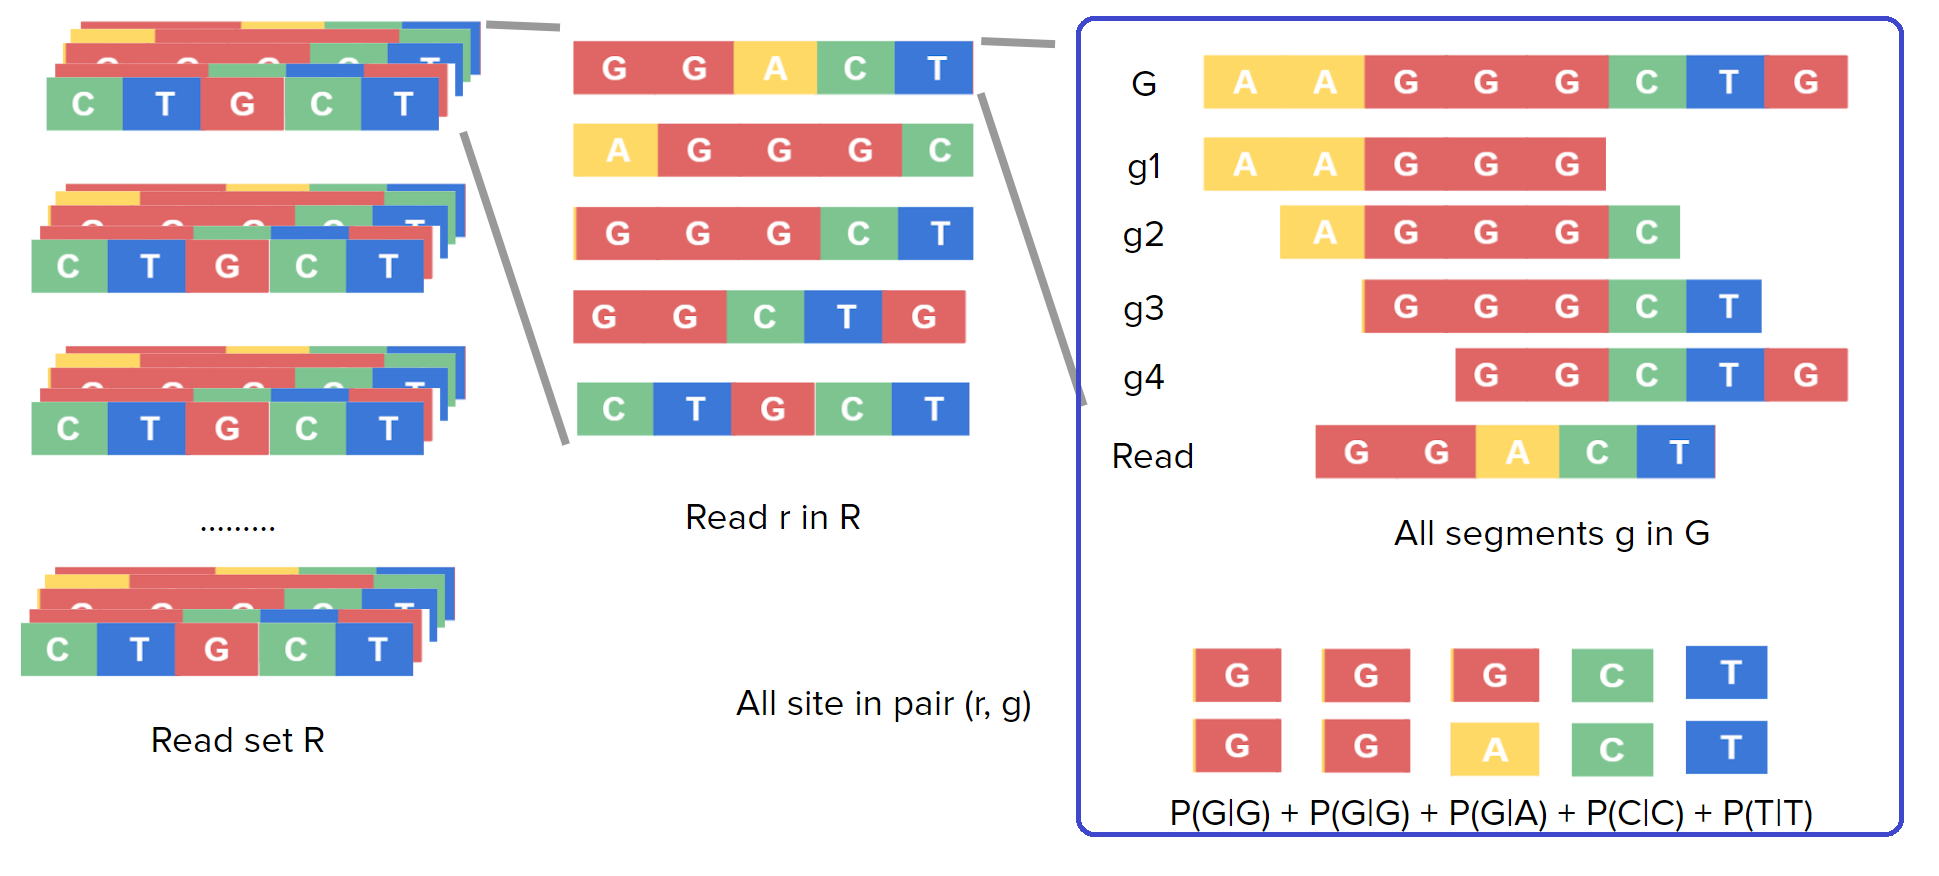
\includegraphics[width=6cm]{figures/overview.png}

\begin{figure}
	\centering
	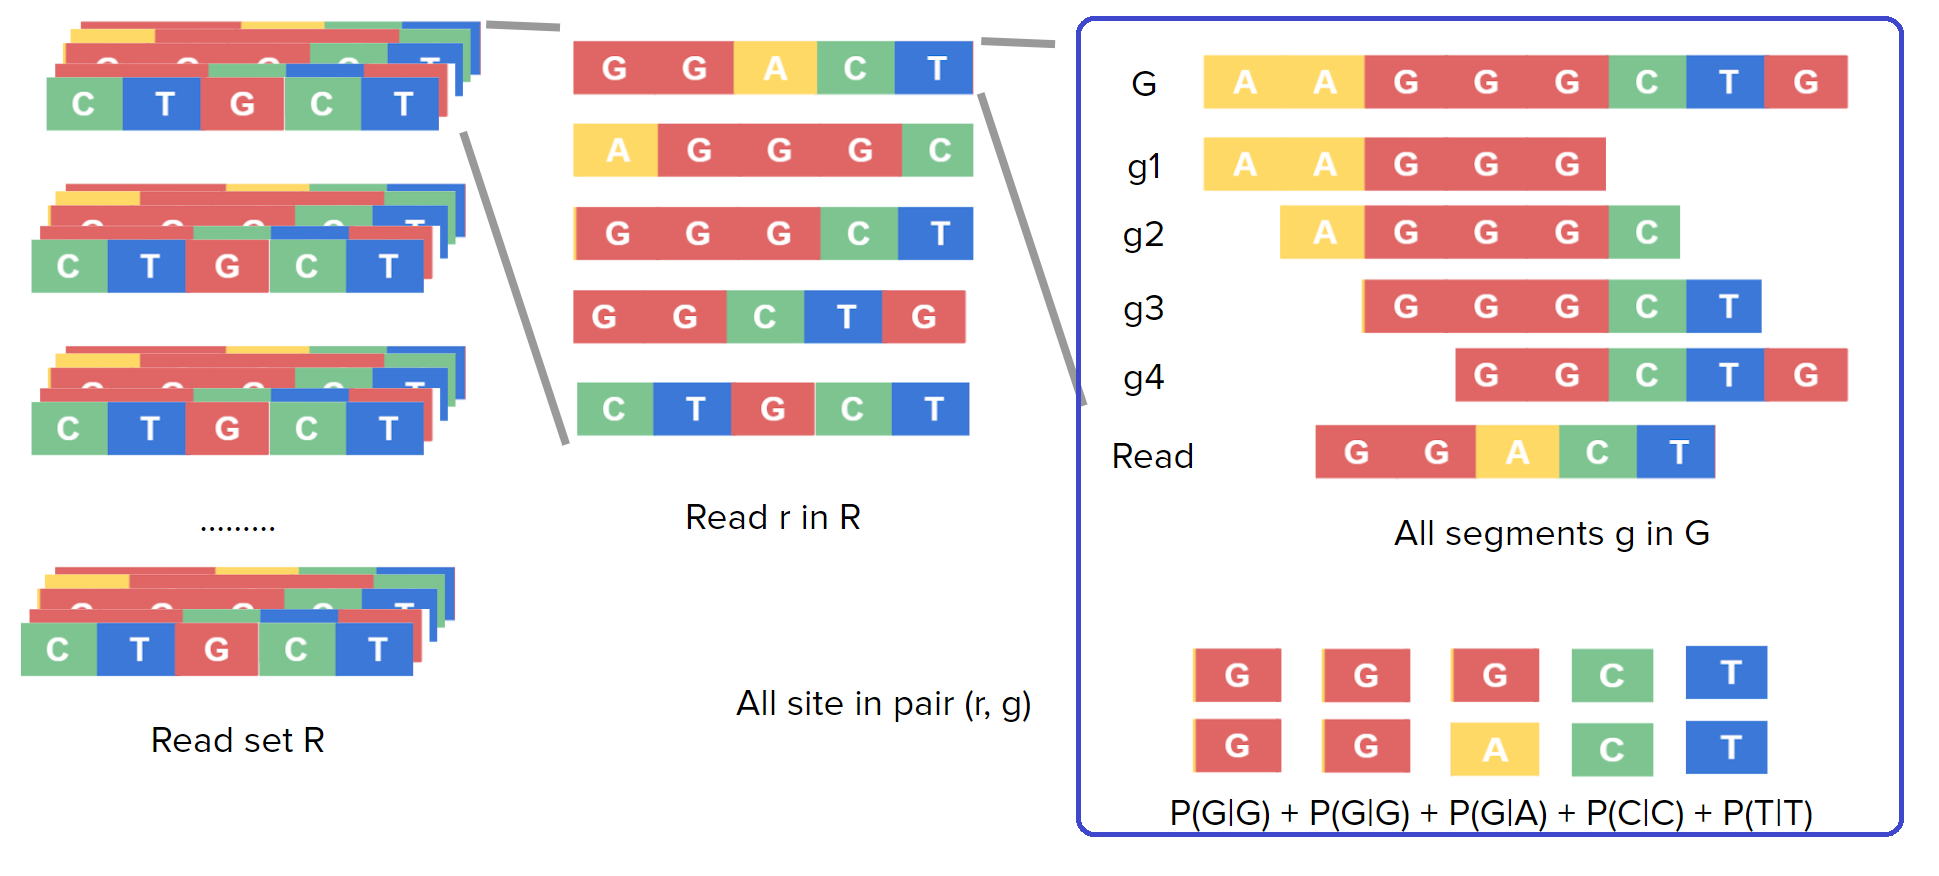
\includegraphics[scale=0.3]{figures/overview.png}
	\caption{Method overview}
	\label{fig:overview} % \ref{this label}
\end{figure}

As shown in Figure \ref{fig:overview}, our goal is to parallelize the parts circled, with the attempt to reduce the total amount of time required to execute the program. We will go through the details in the following section.

\section{Proposed Scheme}
\subsection{CUDA programming model}
Before all else, we should first cautiously design our workflow, trying to acclimate to the CUDA programming model. There exists several essential points to be aware of, which could affect the performance significantly because of the hardware implementations of GPUs. For modern NVIDIA GPUs that support CUDA, often comes with numerous streaming processors(SP), which are the cores on the GPU. Each of them is responsible for executing a thread in our program. They are grouped to form streaming multiprocessors(SM), the basic unit programmers control to execute our parallelized functions, also known as kernels in CUDA terminology. Streaming multiprocessors have their own set of streaming processors, along with their own hardware units such as registers, cache, shared memory, and warp scheduler that schedules warps, the basic unit when it comes to runtime execution. Each warp contains 32 threads, while they share one program counter. Thus, when threads in the same warp executes instructions conditionally, possibly through statements such as if-else, will slow down the process since those threads not executing will be temporarily deactivated, waiting for others to finish. Such problem is refferd to as warp divergence, and could result in a performance loss due to the serialized manner. Another issue that could worsen performance is memory copying. Since kernels launced on GPUs, or device for CUDA terminology, cannot directly access the host memory, those data to be computed should be copied to the device beforehands. However, copying data between host and device is quite time consuming, being likely to take more time than the actual computing operations if not designed carefully. Hence, these are our main concerns during development, while seeking to keep the kernels generalized, ready for further integration. To better demonstrate how the task is designed in a parallel fashion, the pseudocode of the implementation, without parallel computing, is shown below.

We will then describe how we built up the parallelized implementation step by step in the following sections.

\subsection{Computing the likelihood with given genome segment}
First of all, for any given pair of genome segment $g$ and sequence read $r$, the likelihood of the read being sequenced from $g$ is computed by product of the likelihood of all base pairs. Since the likelihood of each base pair match/mismatch is independant to that of other base pairs, they can be computed concurrently. This provides us the oppurtunity to accelerate this process by computing them in parallel, where the maximum number of operations that can be done in parallel is bounded by the length of the read $r$. Considering NGS read data, which is often around 100 to 150 base pairs in terms of read length, we can easily load the entire read onto the GPU and allocate a thread for each base, since the size is rather small in comparison to the memory capacity and the core counts of modern GPUs. A schematic diagram for such process is shown in Figure \ref{fig:prg}.
\begin{figure}
	\centering
	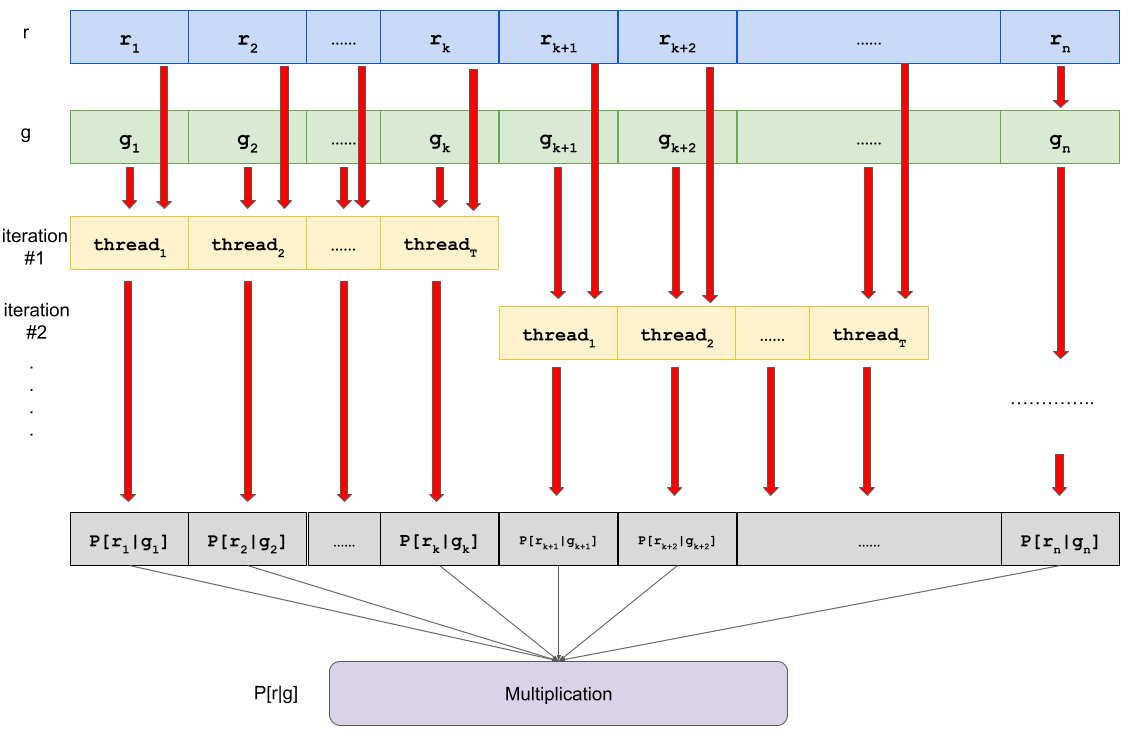
\includegraphics[scale=0.3]{figures/method1.png}
	\caption{Parallel computation for $P[r|g]$}
	\label{fig:prg} % \ref{this label}
\end{figure}


\subsection{Computing the likelihood with given reference genome}
Next, we would like to further extend the degree of parallelism, seeking to utilize the performance provided by the GPU. Here, we take a closer look at the intermediate result, $P[r|G]$. In most cases, knowing the exact genome segment $g$ where read sequence $r$ is sequenced from in advance is unrealistic. Thus, in the original method, for all possible genome segment $g$ sampled from the hypothesis genome $G$, with the exact length with the given read $r$, were considered. $P[r|g]$ are calculated iteratively, with the summation of their results being the final score of the given read. Since the total amount of segments to be considered is related to the length of read sequence (equals to $2*{\ell_r}$), the execution time required grows in polynomial time with the sequence length. Apparently, the results of $P[r|g]$ for different genome segment $g$ is also independant, opening an oppurtunity for parallelism. In addition to the entire read $r$, we also loaded the selected genome $G$ to the GPU, allocating a block of threads for each possible genome segment $g$. Within each block, we execute the same instructions as described in the previous section, calculating the probabilities for each site in their corresponding thread, as shown in Figure \ref{fig:prG}. From the perspective of each thread, the probability they need to compute is illustrated in Figire \ref{fig:tv}.
\begin{figure}
	\centering
	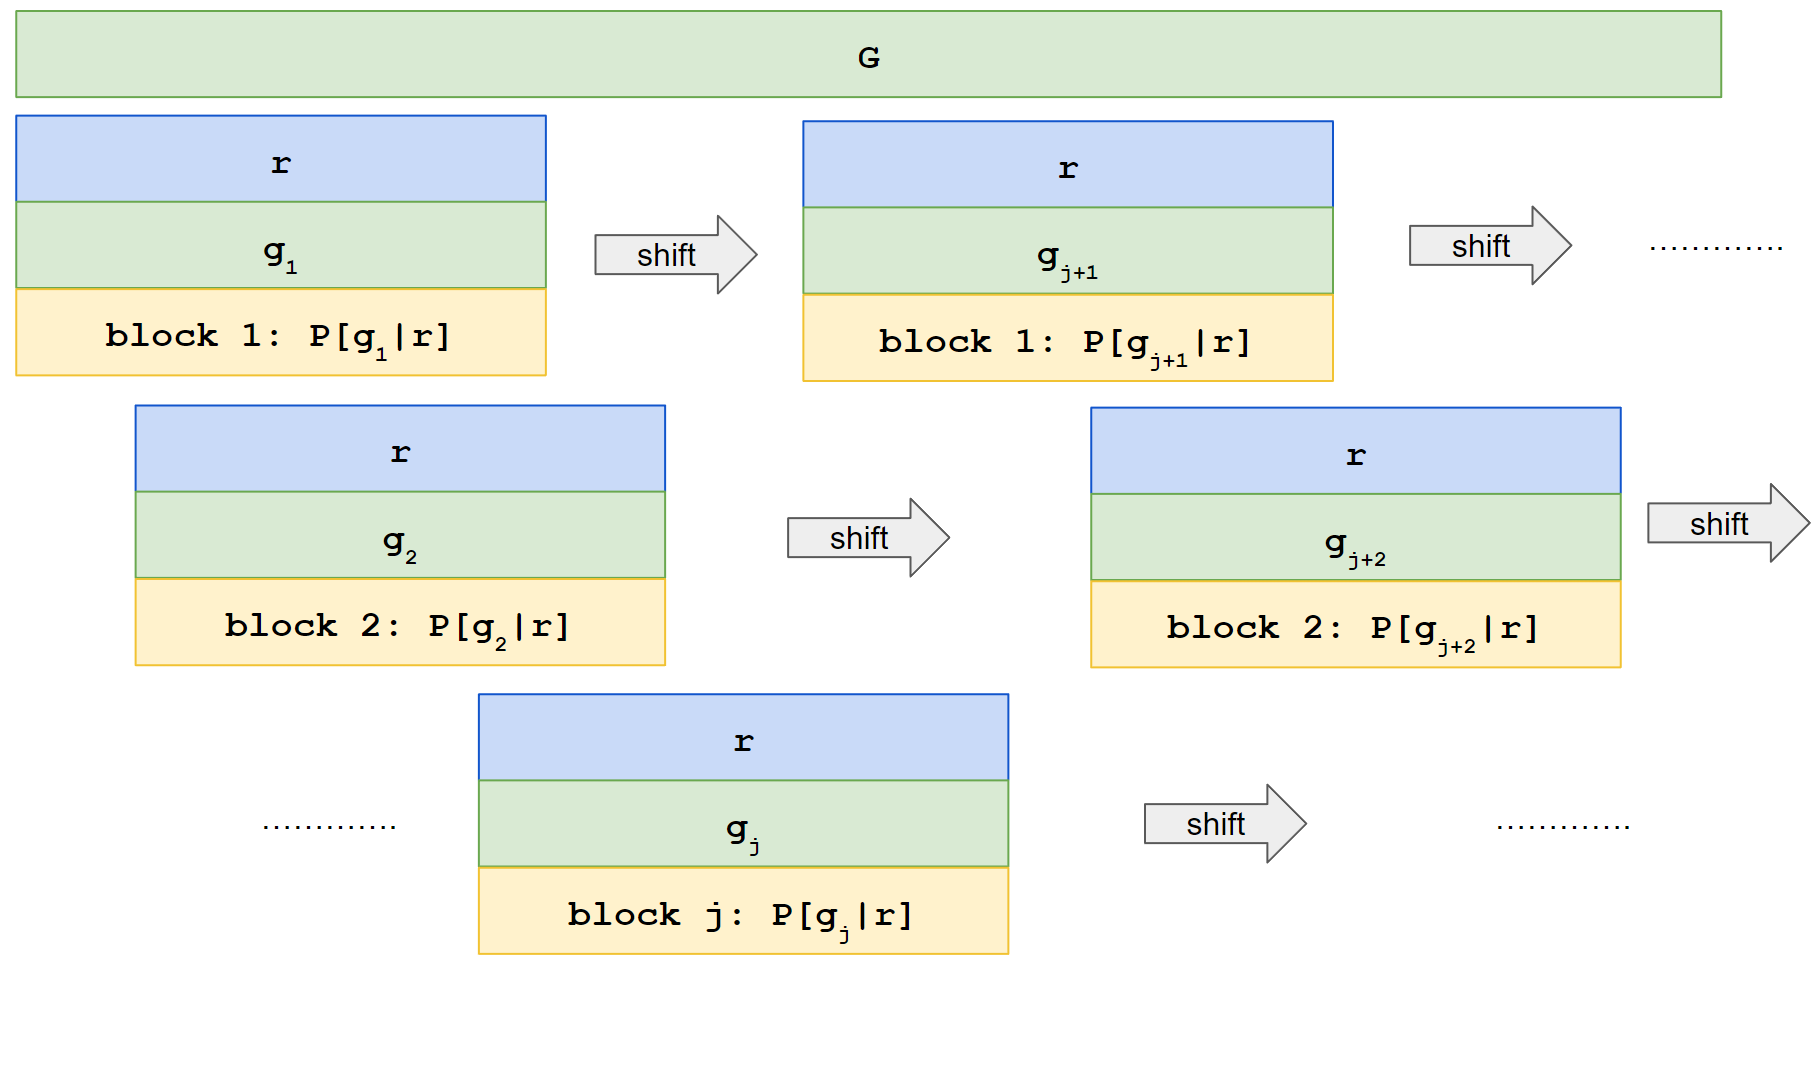
\includegraphics[scale=0.3]{figures/prG.png}
	\caption{Multiple CUDA blocks when parallel computing $P[r|G]$}
	\label{fig:prG} % \ref{this label}
\end{figure}
\begin{figure}
	\centering
	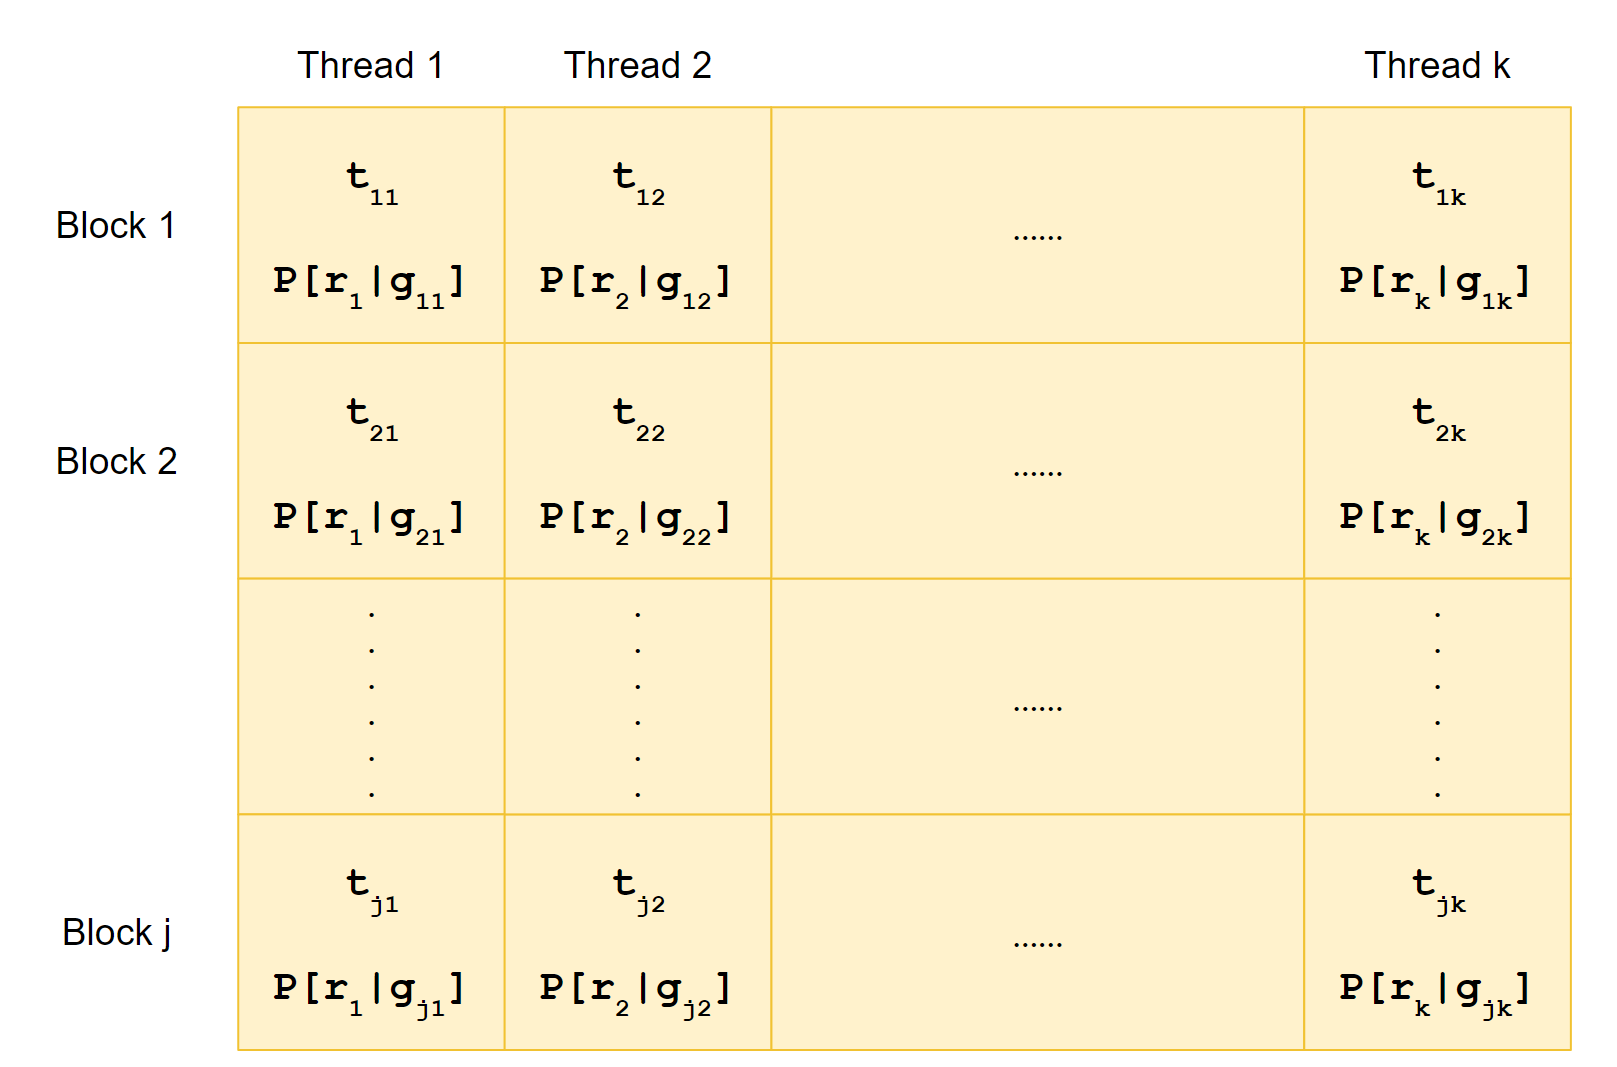
\includegraphics[scale=0.3]{figures/threadview.png}
	\caption{Tasks for each thread when parallel computing $P[r|G]$}
	\label{fig:tv} % \ref{this label}
\end{figure}

Through the above method, we have already reduced the amount of time required to execute the program. This also allows us to revisit a term that was previously ignored: insertion/deletion errors in read sequences. Since indel errors not only modifies the sequence but also introduce shifts, it would increase the time complexity, proportional to the length of reads. With the previous implementation, where the operations were sequentially executed, this would sure intensify the computational cost and lead to longer execution time. Mainly considering generation sequencing data, which has a rather low probability of indel errors in the sequencing phase, an assumption that there was no indel sequencing errors was made, in order to avoid the problem descibed above. However, with the aid of GPUs, such operations can be done concurrently, reducing the amount of time required to compute the final result. In GPU-EAGLE implementation, a threshold value is input by the user, indicating the maximum number of indel errors to be taken into account. After all, the probability of such errors is still fairly low, making it pointless to compute all of the combinations of shifted reads and indels. Knowing the threshold beforehand, all of the possible reads having less indel errors than it is then listed out and assigned to the GPU. Similar to the base case where no indel errors was considered, we would need a block of threads for each pair of read r and genome segment g. With regard to the same read having multiple variations due to the introduced indel errors, the GPU would launch a two dimensional block instead of the original one dimensional block, with the extra dimension representing the index of read in the list of possible reads with indel. To allow such indeled read list to be long exceeding the block size launched, either because of hardware constraints or user settings, the list would be partitioned to batches with the same size as the y dimensional size of the two dimensional block. At last, the results of each batch would be added up to acquire the final result.

\chapter{Results}
\section{Input dataset}
To better compare the results with and without GPU acceleration, an experiment was conducted using the reconstructed diploid sequence of human genome chromosome 22 from hg19 reference sequence, which is one of the dataset that were used in the original study. Intend to investigate possible speedup when facing third generation sequencing read data, simulated sequencing reads with 10,000 base pairs were generated by random sampling from the reference genome. Reads with different lengths were also generated as a reference and an indicator for possible future generation sequencers.

\section{Benchmark platforms}
EAGLE-GPU is compiled with CUDA version 10.1. The experiments were conducted on a machine with a single AMD Ryzen™ 9 5950X desktop processor, consisting of 16 hyper-threaded physical cores running at their base clock 3.4 gigahertz, and 128 GB of random access memory. The GPU installed on the machine is a single NVIDIA GeForce RTX™ 3090 graphics card.

\section{Identical dataset: The NS12911 variants}
First of all, we used the exact same variant dataset that was mentioned in the original EAGLE paper to inspect the performance difference between the sequential and the parallelized implementations. In search of the best grid size and block size settings for this task, we conducted a first experiment disabling the CPU's multithreading setting, measuring the time taken for all combinations of 1, 32, 64, 128, 256, threads and blocks respectively. As we can see in Figure \ref{fig:gpuconfig}, the best configuration would be using 32 blocks per grid, with each block running 32 threads. This results in the program taking 0.342212 hours to finish the task. Later on, attempting to compare the results with and without GPU acceleration, the experiment is then conducted by adopting a single threaded CPU setting, with and without GPU parallel computing under the best kernel launch configuration, gradually moving to a multithreaded setting. The results are shown in Figure \ref{fig:multithread}. For this dataset, the execution time both reduced with the amount of threads increasing, until 8 threads were used. However, we can see that with the current implementation of GPU computing, the execution time is not effectively reduced, but is somehow worsened instead.
\begin{figure}
	\centering
	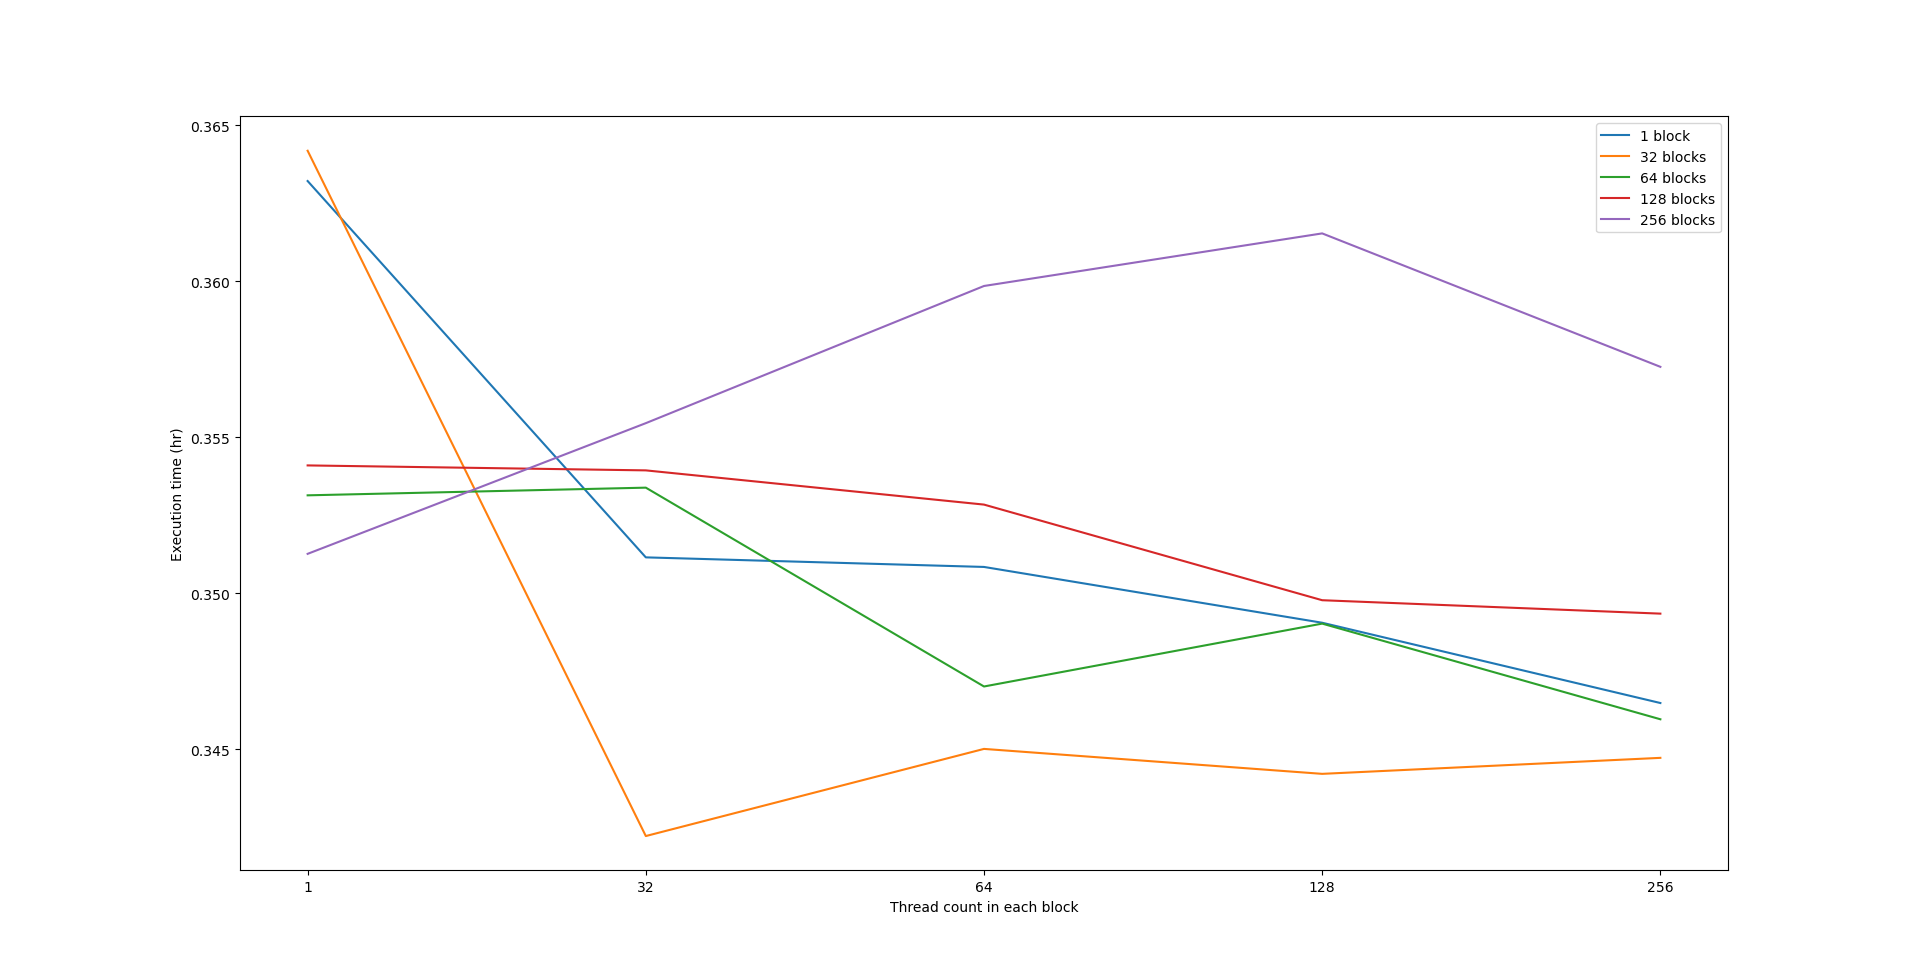
\includegraphics[scale=0.3]{figures/gpu_config.png}
	\caption{Time taken for different kernel launch configuration}
	\label{fig:gpuconfig} 
\end{figure}
\begin{figure}
	\centering
	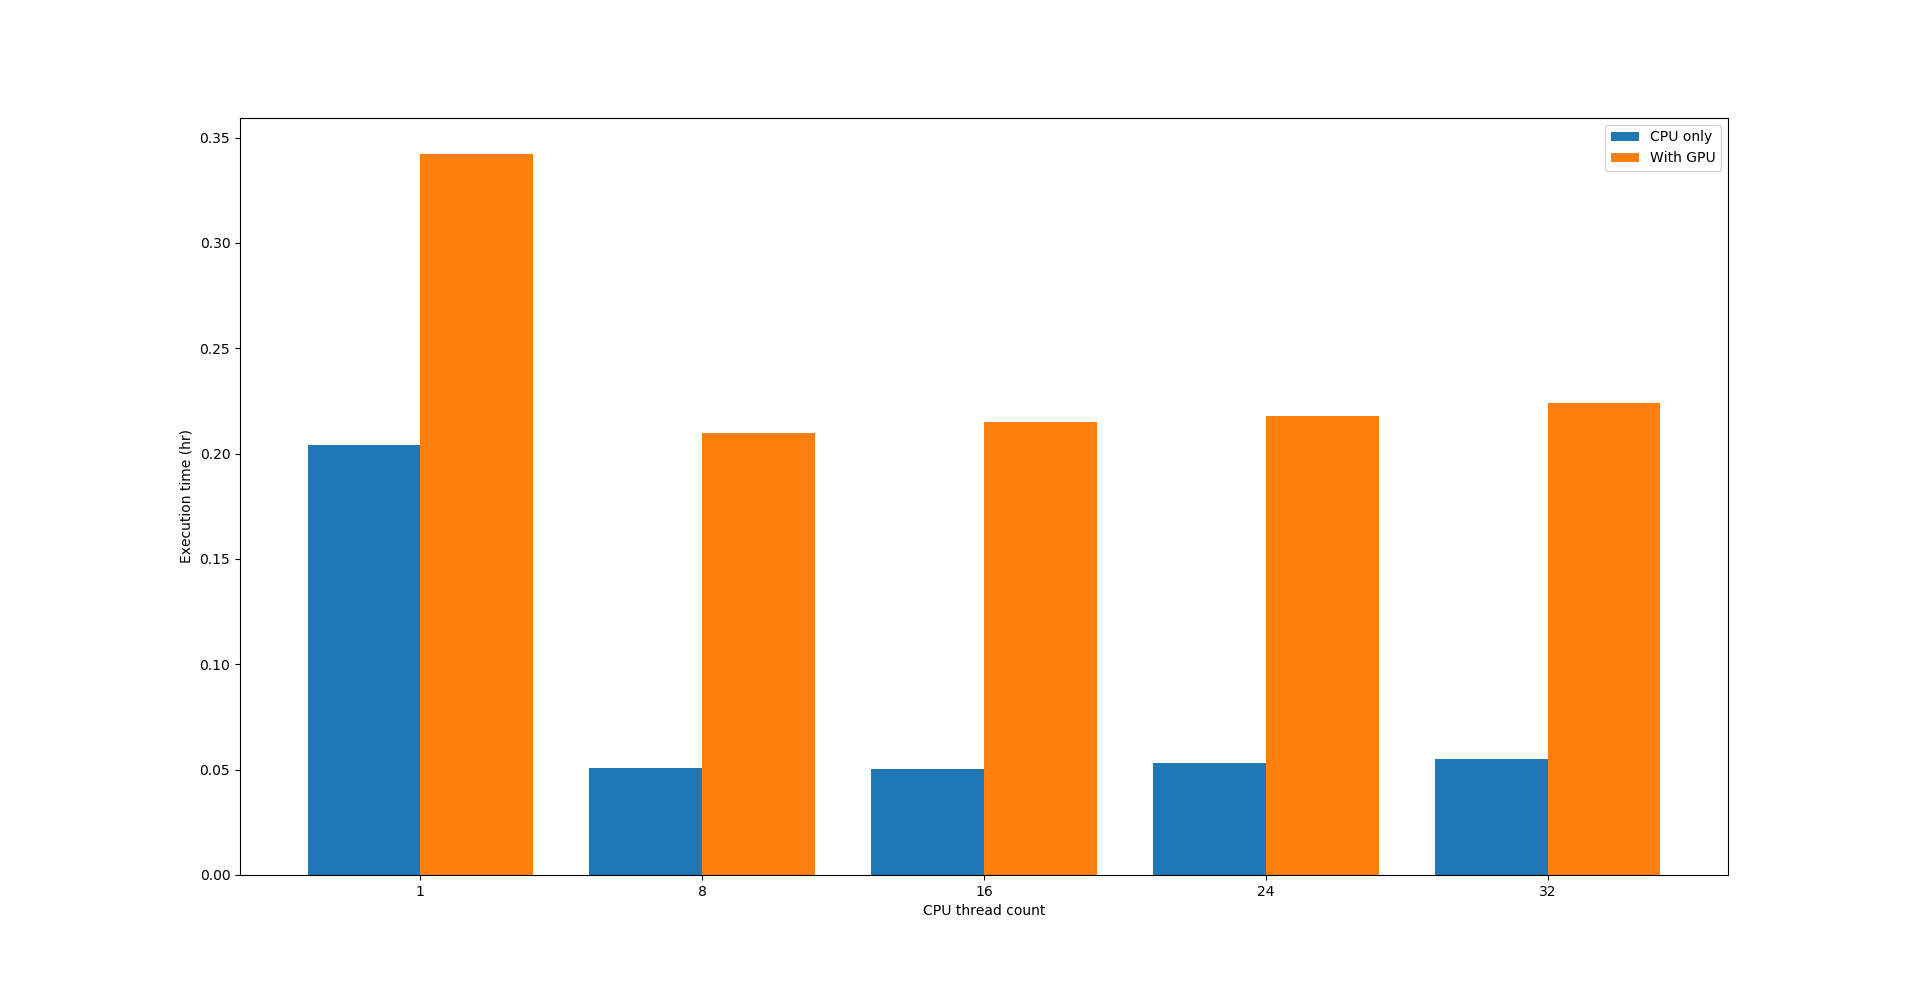
\includegraphics[scale=0.3]{figures/multithread.png}
	\caption{Time taken for different CPU threading settings}
	\label{fig:multithread} 
\end{figure}

\section{Simulated reads with different lengths}
With the length of the sequenced reads growing considering third generation sequencing, we performed another experiment, with the intention to figure out the relations between parallelism and sequence length. We did not only test with sequences with around 10000 bp which is the most common length for Nanopore sequencing results, but also other varying lengths, preparing our tool in advance for possible futeure sequencing technologies which might produce reads in varying lengths. Simulated reads were generated, with different lengths, by randomly sampling from the reference genome. Concentrating on the performance difference regarding the presence of GPU acceleration only, we performed this experiment in a single CPU threading setting, with 256 blocks x 256 threads kernel launch configuration. Clearly seen in Figure \ref{fig:readlen}, the execution time without GPU acceleration dramatically increases with the read length, while that of GPU accelerated version growing rather mild, outperforming the other after reads expand over 1000 base pairs.
\begin{figure}
	\centering
	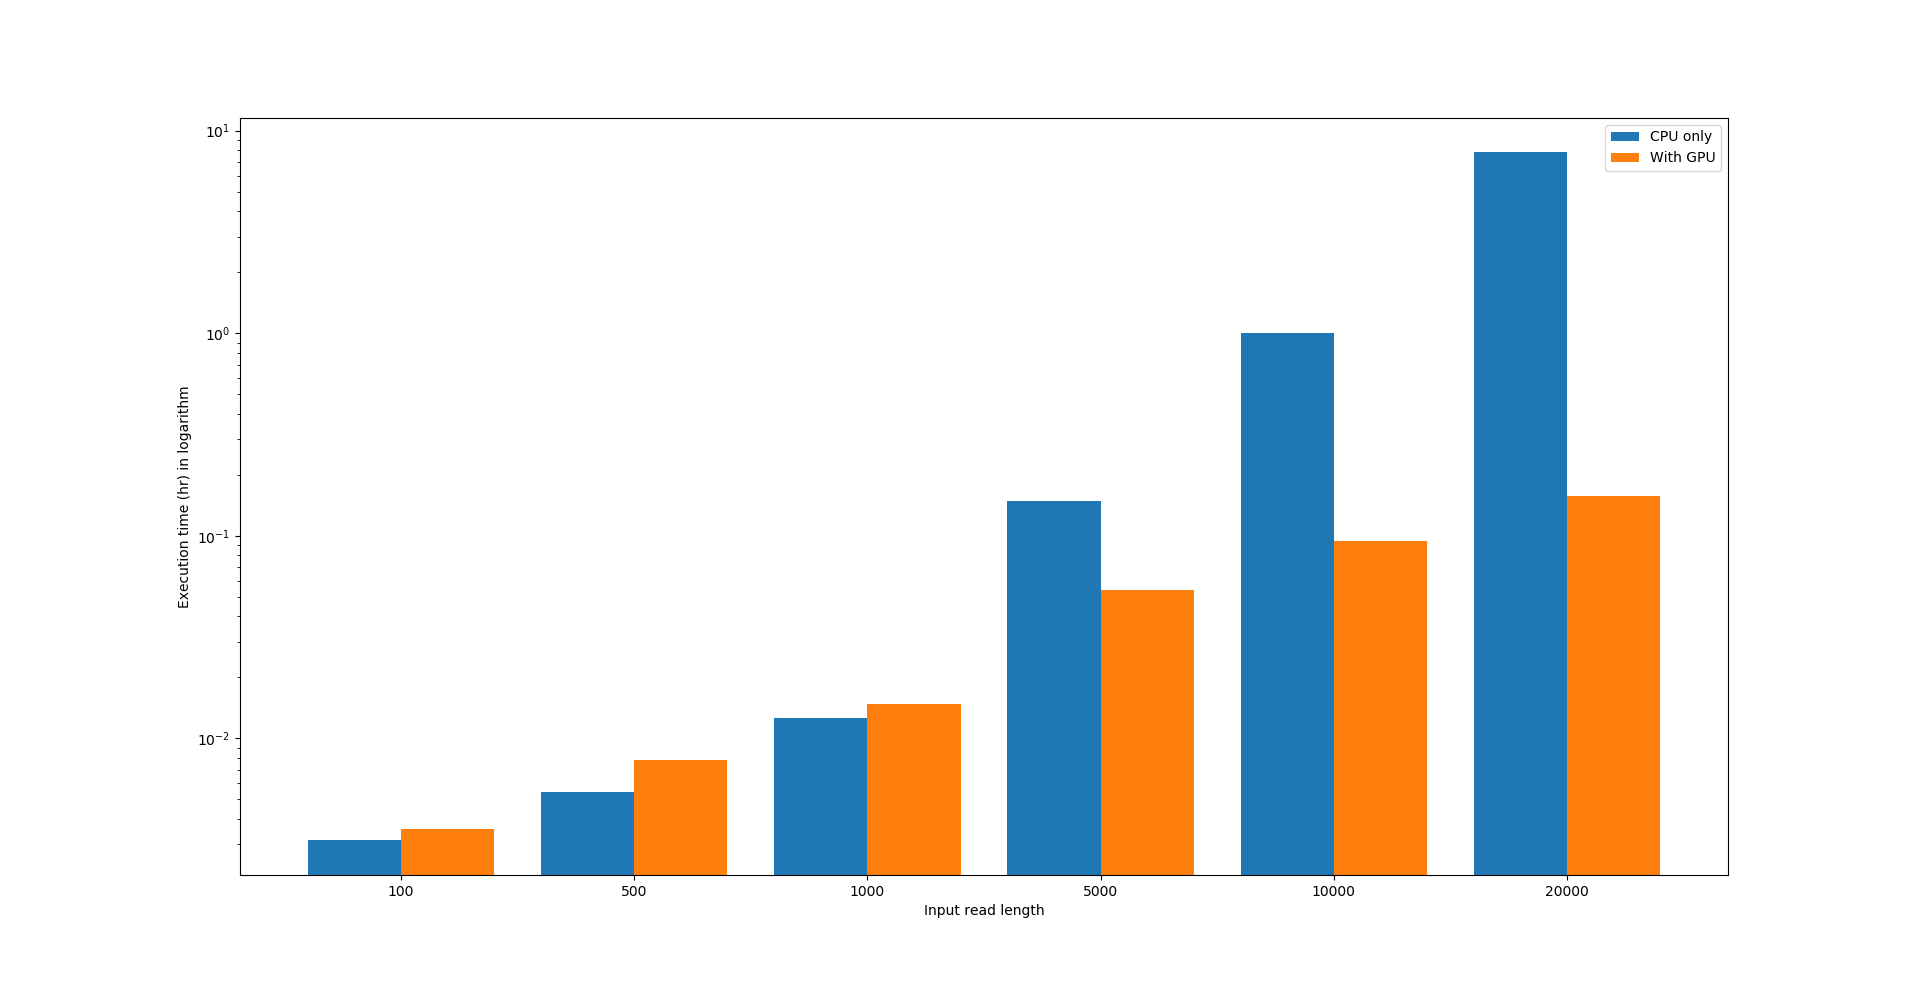
\includegraphics[scale=0.3]{figures/readlen.png}
	\caption{Execution time for different input read lengths}
	\label{fig:readlen} 
\end{figure}

\section{Considering read indel errors}
Attempting to find out if the consideration of indel errors is feasible, although computationally expensive, with the assistance of GPU parallel computing, we reused the NS12911 dataset, but without any assumption about the presence of read indel errors. Instead, a threshold is issued, while all of the reads with indel errors length within the threshold is considered. As mentioned in the previous study, doing so with CPU only is extremely time-consuming, thus we had to set a limitation for the threshold, not exceeding 1, in order to regulate the total execution time to a reasonable extent. As we can see in Figure \ref{fig:readindel}, a positive result of GPU speedup is achieved even with one possible read indel error, not to mention computing even more combinations of indels for a larger threshold.
\begin{figure}
	\centering
	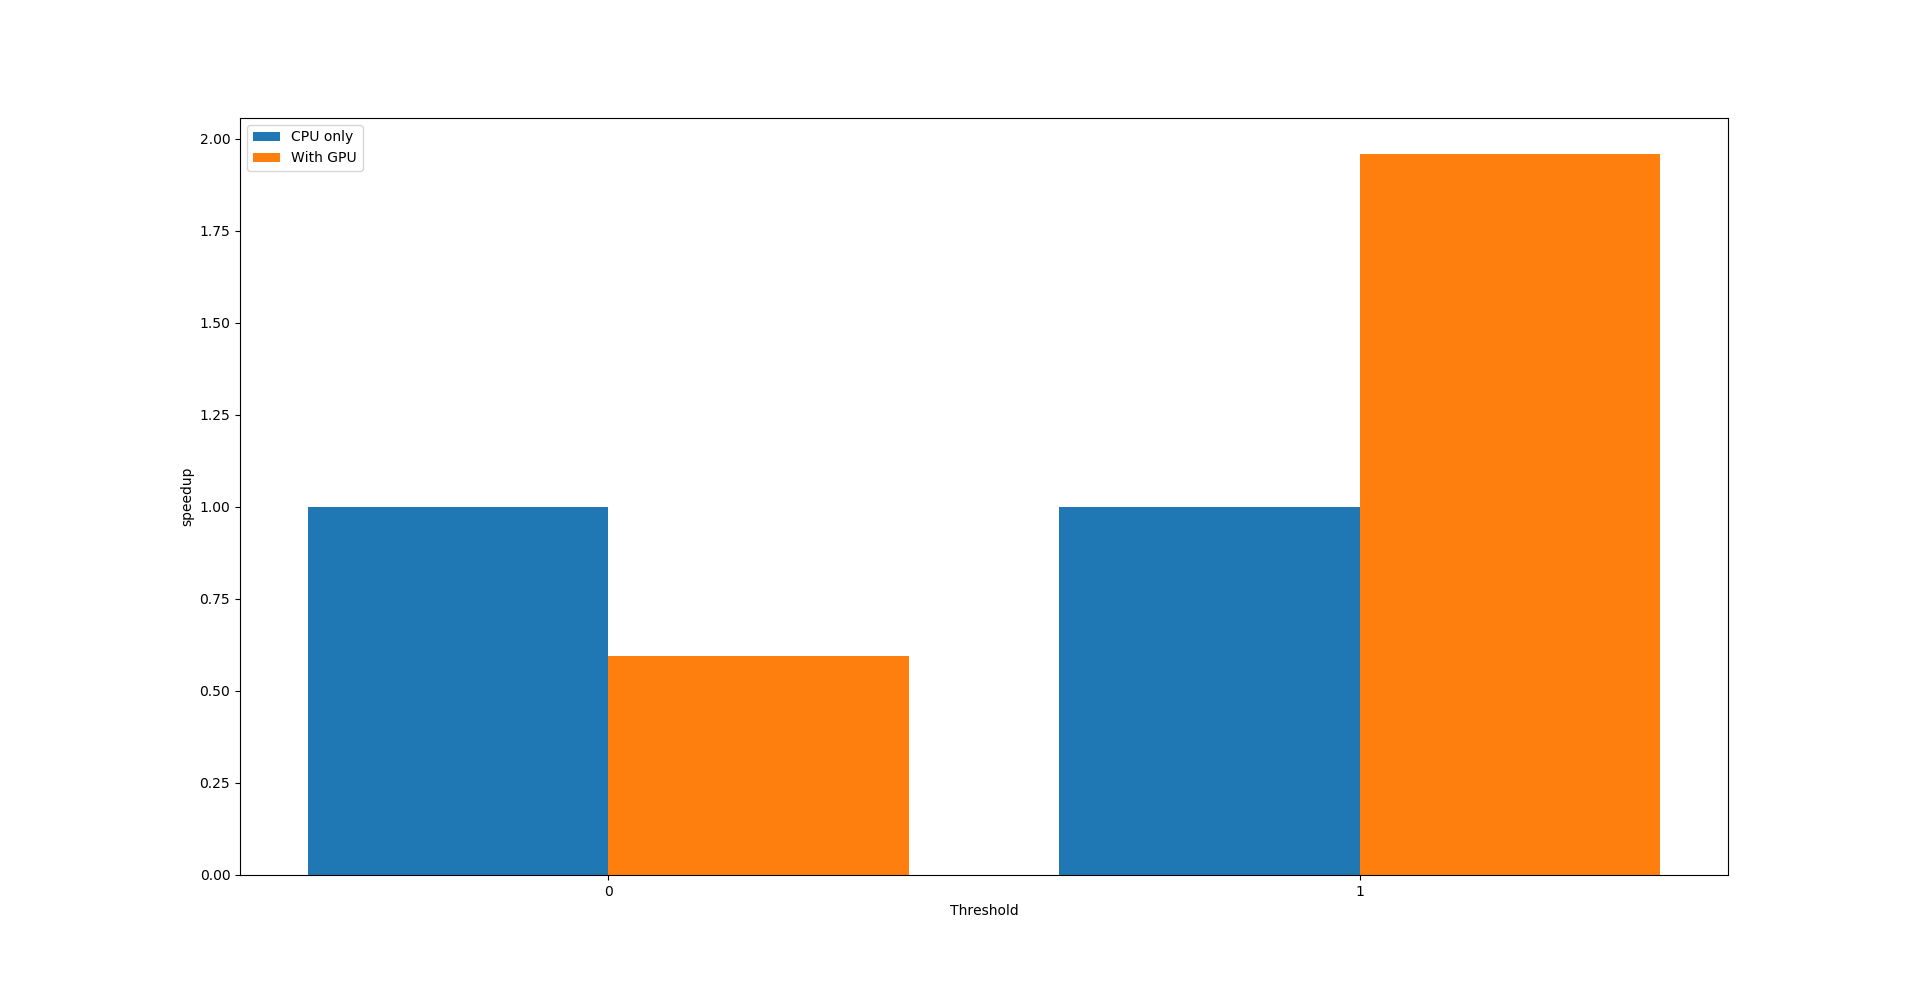
\includegraphics[scale=0.3]{figures/read_indel.png}
	\caption{Time taken for different CPU threading settings}
	\label{fig:readindel} 
\end{figure}

\chapter{Discussion}
EAGLE-GPU is a GPU accelerated implementation of the previously published method, EAGLE, while maintaining similar data processing workflow for better integration with the previous tool. Being generalized by re-engineering the fundamental functions, without packing the entire algorithm into a hard coded GPU kernel sure helps with flexibility, preparing the tool for further applications. However, performance were sacrificed to a certain extent by doing so. In the following sections, we would like to discuss our interpretation of the experimental results, along with possible approaches to further increase the speedup.

\section{Case study: The original dataset}
As mentioned in the previous chapter, we can easily see that applying GPU computation does not benefit the results when the dataset tested in the previous research was used. Through observations of the profiling results, it is clear that the computational time, excluding the time for data copying between host and device, is longer for GPUs, not to mention data copying adds up to the total execution time if GPU is used. The main reason for this is that, although equipped with a lot more processors, the computational power of a single GPU core is weaker than that of a CPU core. As a consequence, if the extent of parallelism was not high enough, distributing tasks to the GPU could possibly become a drawback when it comes to execution time. To better illustrate such problem, a rather easy experiment was made, which is the addition of two vectors, with the execution time measured for different vector sizes. The results are shown in Figure \ref{fig:cpugpuvec}.
\begin{figure}
	\centering
	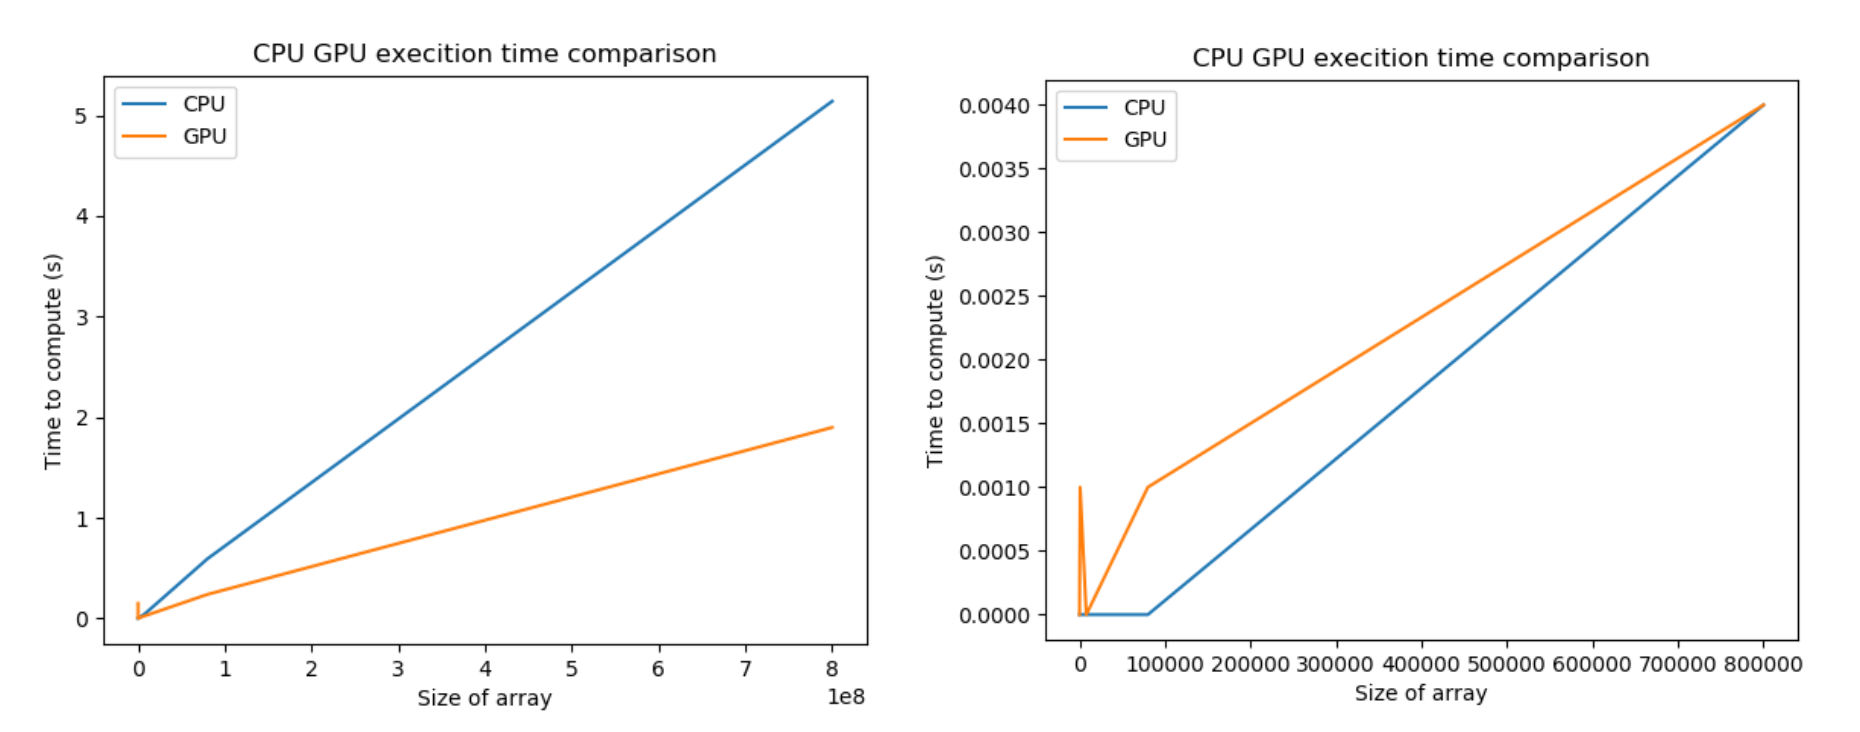
\includegraphics[scale=0.3]{figures/cpugpu_vector.png}
	\caption{Comparing the performance between CPU and GPU}
	\label{fig:cpugpuvec} % \ref{this label}
\end{figure}
As we can see in Figure \ref{fig:cpugpuvec}, applying GPU acceleration is not favoring until the size of vector exceeds 800000. Now we further inspect our dataset, where all of the sequencing reads have a length of 100 bp. When we calculate $P[r|G]$, a total of 100 x 100 = 10000 operations can be executed concurrently, each computing the probability at a certain cite. Although the time taken between addition and querying the probability of a DNA base might differ, but the considerable difference between the two numbers leads us to infer that the reads in this specific dataset is too short for it to be profitable when it comes to GPU computation. Such supposition could be confirmed with the second experiment, which we would further discuss in the next section. As a result, we suggest to not apply GPU acceleration when handling datasets with shorter reads. Since the instructions performed recurrently are rather little, the CPU can effectively finish the job solely, without needing any help from the GPU. The only condition we could think of that GPU acceleration would be profitable with short reads is when numerous reads maps to a single interval of interest. Under this circumstance, implementing a specialized kernel, computing $P[R|G]$, where $R$ denotes the set of reads, could be a practical approach. However, the main objective for this research is to build a rather general solution, for future applications to build on, thusly this will be left as a possible future work, which can be conducted in a similar fashion if such type of data is encountered.

\section{Case study: Simulated TGS read data}
By conducting this experiment, we could not only validate the pressumption discribed in the previous section, but also acquire an estimation of the possible speedup when applying EAGLE-GPU to third generation sequencing data. Here, we can easily see that the speedup performance gradually increases as the size of sequenced reads grow, surpassing it of the CPU when the read length passes 1000 bp. This sure supports our pressumption, concluding that GPU acceleration is a favorable option when it comes to third generation sequencing, or even further sequencing technologies with sequencing read lengths beyond 1000 bp.

\section{Case study: Read indel errors}
The execution time dramatically increases when read indels are taken into consideration, justifying the attempt to ignore such errors in the previous work. With the aid of GPUs, such difficulty could be tackled, to a certain extent. As long as it fits into the device memory, we can load all possible reads, including different combinations of indels, onto the GPU. They can be computed concurrently, greatly reducing the time required for such operations, despite being computationally expensive. With the threshold adjustable, GPU acceleration could come in as a relief if the sequencing technology is reported to have a noticeable read indel issue.

\section{Future Work}
Trying to investigate various possibilites of application for GPU to improve the performance, this paper provides the implementations of the general usage functions in CUDA. Unlike programs executed particularly on CPU, the design of GPU kernels often require extra attention, including memory copying schema and the detail implementation of algorithms. If we peurely consider datasets with shorter sequencing reads, the extent of parallelism could be further increased by computing different read sets concurrently. With a specific kernel for each case, warp divergence could be eliminated. Theoretically, this could benefit cases when the dataset consist of large amount of read sets, enormously reducing the amount of time to evaluate the likelihood by computing the results for each set all at once. Another possible optimization would be lessening the memory copying cost. Despite it not being the bottleneck of the program, some advanced techniques could be applied to lower the amount of data copied between the host CPU and the device even more. For example, if we are targeting only DNA and RNA sequences but not proteins, we could easily represent the bases, A, C, G, T(U for RNA), N, in 3 bits. Thus, instead of copying them as characters, they could be encoded first, enabling us to pack 2 bases into one unsigned integer. This is a common trick among sequencing related GPU applications, also adopted by other tools such as GASAL2 and NVBIO.

\chapter{Conclusion}
In this paper, we propose and implemented a GPU accelerated version of EAGLE, a previously proposed method for alternative genome likelihood evaluation. GPU-EAGLE utilizes the massively parallel architecture of modern GPUs, enabling instructions to be executed concurrently on multiple different data. This prepares the original method for the continuous growth when it comes to the size of sequencing data. Besides, we also investigated the feasibility of taking sequencing read indel errors into consideration, which is computational expensive and used to be ignored, after increasing the program throughput by applying parallel computation. We provide experimental results showing that GPU-EAGLE outperforms the CPU version when the data size is large enough, and conclude that designing a specialized GPU kernel could always be an option for forthcoming applications with excessive computational operations.

\newpage
\AddToContents{References}
\printbibliography


\end{document}
